%!TEX program = xelatex
% !Mode:: "TeX:UTF-8"
%% 请使用 XeLaTeX 编译本文.
\documentclass[smd,forlib,entitle]{NJTECHMaster}   % 选项 forprint: 交付打印时, 建议加上此选项, 以消除彩色链接文字, 避免彩色字迹打印偏淡.
                                              % 选项 forlib: 提交给图书馆的电子版, 需要加上选项 forlib, 以消除空白页和彩色链接.
                                              % 选项 smd: Specialist Master's Degree, 产生专业硕士学位论文封面、页眉.
                                              % 选项 entitle: 使下文的\sidetitle选项生效,尽量不要在中文标题中带英文,对齐还有点小问题.
%%%=== 参考文献=== %%%
\bibliographystyle{abbrv}        % 参考文献样式,  plain,unsrt,alpha,abbrv 等等
%%%%%%%%%%%%%%%%%%%%%%%%%%%%%%%%%%%%%%%%%%%%%%%%%%%%
\begin{document}
%%%%%%%-------------------------------------------------

\fenleihao{}  % 分类号:《中国图书资料分类法》的类号. 必填. 要根据自己的学科方向填写!!
\miji{}                % 密级
\UDC{}               %《国际十进制分类法UDC》的类号. 选填.
\bianhao{}  % 学校编号, 10291是南京工业大学的编号


\title{南京工业大学硕士论文~\LaTeX~模板}
\sidetitle{南京工业大学硕士论文L  A T E X 模板}%边栏的标题,手动将英文字母空格分开,不启用entitle选项时可忽略
\Etitle{A \LaTeX~Thesis Template for NanjingTech University} % 英文题目
\author{郭索眸}
\Eauthor{Suomou Guo}            %作者英文名
\Csupervisor{赵志宏\quad 教授}        %指导教师中文名、职称
\Esupervisor{Prof.~ZHAO Zhi Hong}     %指导教师英文名、职称
\Cmajor{计算机技术}                          % 一级专业中文名[ SMD:领域名称]
\Cspeciality{工程硕士}                     % 二级学科名称[ SMD:工程硕士]

\date{2022年4月}                    % 硕士类只写年月. 要注意和英文日期一致!!
\Edate{April, 2022}                   % 英文封面日期

%-----------------------------------------------------------------------------
\pdfbookmark[0]{封面}{title}         % 封面页加到 pdf 书签
\maketitle
%-----------------------------------------------------------------------------
% !Mode:: "TeX:UTF-8"

%%% 此部分包含: (1) 英文封面 (无需改动) ; (2) 郑重声明 (无需改动) ; (3)项目资助(需要自己填写) .

%%%%%%%%%%%%%%%%%%%%%%%%%%%%%
%%% -------------  英文封面 (无需改动)-------------   %%%
%%%%%%%%%%%%%%%%%%%%%%%%%%%%%
\thispagestyle{empty}
\renewcommand{\baselinestretch}{1.5}  %下文的行距
\vspace*{0.5cm}
\setmainfont{Times New Roman}

\begin{center}{\zihao{3} \textbf{\MakeUppercase{\the\Etitle}} \par}\end{center}

\vspace*{25mm} %插入空白
%\vfill

\begin{center}
\zihao{3}
A Thesis Submitted to\\
Nanjing Tech University\\
For the Professional Degree of Master of\\
Engineering\\

\vspace*{20mm} %插入空白

By\\
{\sc \the\Eauthor}      \\

\vspace*{20mm} %插入空白

Supervised by\\
{\sc \the\Esupervisor}\\


\vspace*{25mm} %插入空白

\the\Edate

\end{center}
%%%%%%%--判断是否需要空白页-----------------------------
  \iflib
  \else
  \newpage
  \thispagestyle{empty}
  \cleardoublepage
  \fi
  
  
%%%%%%%-------------------------------------------------
%%%--- 加入``郑重声明'' --- %%%%%%%%%%%%%%%%%
{
	\pagestyle{empty}
	\newpage
	%\setlength{\parindent}{0pt} %
	\vspace*{20pt}
	\begin{center}{\zihao{3}\songti \textbf{学位论文独创性声明}}\end{center}
	\par\vspace*{30pt}
	\renewcommand{\baselinestretch}{2}
	{\zihao{-4} \songti %
		
		
		\noindent 本人声明所呈交的学位论文是我个人在导师指导下进行的研究工作及取得的研究成果。尽我所知,除了文中特别加以标注和致谢的地方外,论文中不包含其他人已经发表或撰写过的研究成果,也不包含为获得南京工业大学或其它教育机构的学位或证书而使用过的材料。与我一同工作的同志对本研究所做的任何贡献均已在论文中作了明确的说明并表示了谢意。\\
		\begin{tabular}{lp{3cm}p{0cm}lp{3cm}l}
			\raisebox{-0.5ex}[0pt]{\makebox[2.5cm][s]{研\hfill 究\hfill \hfill 生\hfill 签\hfill 名:}} & {}\hfill\raisebox{-0.5ex}[0pt]{}\hfill{} &  &
			\raisebox{-0.5ex}[0pt]{\makebox[2.5cm][s]{日\hfill 期:}} & {}\hfill\raisebox{-0.5ex}[0pt]{}\hfill{} & \\\cline{2-2}\cline{5-5}
		\end{tabular}
		
		
		\vskip2cm
		\par
	}
	
	\begin{center}{\zihao{3}\songti \textbf{学位论文的使用声明}}\end{center}
	\par\vspace*{30pt}
	\renewcommand{\baselinestretch}{2}
	{\zihao{-4} \songti %
		
		
		{\zihao{-1} \noindent $ \square  $}{\zihao{-2} \noindent 1、}南京工业大学、国家图书馆、中国科学技术信息研究所、万方数据电子出版社、中国学术期刊(光盘版)电子杂志社有权保留本人所送交学位论文的复印件和电子文档,可以采用影印、缩印或其他复制手段保存论文并通过网络向社会提供信息服务。论文的公布(包括刊登)授权南京工业大学研究生部办理。(打钩生效)\\
		{\zihao{-1} \noindent $ \square  $}{\zihao{-2}  2、}本论文已经通过保密申请,请保留三年后按照第一项公开(打钩生效)\\
		{\zihao{-1} \noindent $ \square  $}{\zihao{-2}  3、}本论文已经通过校军工保密申请,不予公开(打钩生效)\\
		\begin{tabular}{lp{3cm}p{0cm}lp{3cm}l}
			\raisebox{-0.5ex}[0pt]{\makebox[2.5cm][s]{研\hfill 究\hfill \hfill 生\hfill 签\hfill 名:}} & {}\hfill\raisebox{-0.5ex}[0pt]{}\hfill{} &  &
			\raisebox{-0.5ex}[0pt]{\makebox[2.5cm][s]{导\hfill 师\hfill 签\hfill 名\hfill :}} & {}\hfill\raisebox{-0.5ex}[0pt]{}\hfill{} & \\\cline{2-2}\cline{5-5}
			\raisebox{-0.5ex}[0pt]{\makebox[2.5cm][s]{日\hfill 期:}} & {}\hfill\raisebox{-0.5ex}[0pt]{}\hfill{} &  &
			\raisebox{-0.5ex}[0pt]{\makebox[2.5cm][s]{日\hfill 期:}} & {}\hfill\raisebox{-0.5ex}[0pt]{}\hfill{} & \\\cline{2-2}\cline{5-5}
		\end{tabular}
	
	%%%%%%%-------------------------------------------------
	%%%--- 加入``项目资助'' --- %%%%%%%%%%%%%%%%%
		\clearpage
		\vspace*{20pt}
		\vfill
		\noindent 本文工作得到以下项目资助:
		\begin{enumerate}[1. ]
			\item 国家自然科学基金项目“链路相关无线网络中基于网络编码的数据分发机制研究”(项目编号:61502230);
			\item 江苏省自然科学基金项目“面向无线数据分发应用的新型网络编码机制研究”(项目编号:BK20150960);
		\end{enumerate}
		
	
	
	%%%%%%%--判断是否需要空白页-----------------------------
	\iflib
	\else
	\newpage
	\cleardoublepage
	\fi
	%%%%%%%-------------------------------------------------
}

\renewcommand{\baselinestretch}{1.6}
\small\normalsize




    % 加入英文封面
\frontmatter
\pagenumbering{Roman}               % 正文之前的页码用大写罗马字母编号.

\cleardoublepage
\newpage  
\pagestyle{fancy} \fancyfancy
%------------------------------------------------------------------------------
% !Mode:: "TeX:UTF-8"

%%% 说明: 此部分需要自己填写的内容:  (1) 中文摘要及关键词 (2) 英文摘要及关键词

%%%%%%%%%%%%%%%%%%%%%%%
%%% ------------ 中文摘要 ---------------%%%
%%%%%%%%%%%%%%%%%%%%%%%
\begin{cnabstract}
	
\thispagestyle{onlytitle}

本文主要介绍和讨论了南京工业大学硕士毕业论文的~\LaTeX~模板.
指明了编译方法, 强调了公式排版的一些细节问题, 也指出了一些常见的排版错误.



\end{cnabstract}

\vspace*{10mm} %插入空白

%%%--------- 关键词 -------- %%%
\cnkeywords{毕业论文 \qquad \LaTeX{}\qquad 模板\qquad XeLaTeX }

%%%%%%%%%%%%%%%%%%%%%%%


%%%%%%%%%%%%%%%%%%%%%%%
%%% ------------ 英文摘要 ---------------%%%
%%%%%%%%%%%%%%%%%%%%%%%
\begin{enabstract}
\thispagestyle{onlytitle}
This thesis is a study on the theory of \dots.




\end{enabstract}
\vspace*{10mm} %插入空白
%%%------ 英文关键词 ------- %%%
\enkeywords{Graduation thesis;\LaTeX{};Template;XeLaTeX}


      % 加入中英文摘要.
%---把目录加入到书签---%%%%%%%%%%%%%%
\pdfbookmark[0]{目录}{toc}%%%%%%%%%%%%
\tableofcontents
\thispagestyle{onlytitle}
\addcontentsline{toc}{chapter}{目\texorpdfstring{\quad}{} 录}
%------------------------------------------------------------------------------
\mainmatter %% 重新计算页码,以下是正文
\baselineskip=20pt  % 正文行距为 20 磅
%%%%%%%%%%%%%%%%%%%%%%%%%%%%%%%%%%%%
\chapter{先说重要的}

\section{具体使用步骤}
\begin{description}

  \item[Step 1]  进入 includefile 文件夹\@title,  打开 midmatter.tex,  backmatter.tex 这两个文档,
        分别填写 (1) 中文摘要、英文摘要, (2) 致谢.

  \item[Step 2]  打开主文档 MasterTemplate.tex, 填写题目、作者等等信息, 书写正文.

  \item[Step 3]  使用 XeLaTeX 编译. 具体见 \ref{sec-compile} 节.


\end{description}




\section{编译的方法}\label{sec-compile}

默认使用 XeLaTeX 编译, 直接生成~pdf 文件.



若另存为新文档, 请确保文档保存类型为 \verb|:UTF-8|. 当然目前很多编辑器默认文字编码为 UTF-8.
WinEdt 9.0 之后的版本都是默认保存为 UTF-8 的.



\section{文档类型选择}
文档类型有 3 种情形:

\begin{table}[ht]\centering
\begin{tabular}{ll}
\hline
   \verb|\documentclass{WHUMaster}|                 &  硕士论文 \\
   \verb|\documentclass[forprint]{WHUMaster}|    &  硕士论文打印版  \\
   \verb|\documentclass[forlib]{WHUMaster}|       &  硕士论文图书馆提交版  \\
\hline
\end{tabular}
\end{table}

另外: 专业硕士毕业论文, 请在上述情形另外加上选项 smd. 专业硕士毕业论文的封面稍有不同(中英文封面), 页眉也顺势改变了. 即
\begin{table}[ht]\centering
\begin{tabular}{ll}
\hline
   \verb|\documentclass[smd]{WHUMaster}|               &  专业硕士论文 \\
   \verb|\documentclass[smd,forprint]{WHUMaster}|    &  专业硕士论文打印版  \\
   \verb|\documentclass[smd,forlib]{WHUMaster}|       &  专业硕士论文图书馆提交版  \\
\hline
\end{tabular}
\end{table}



相关解释见接下来的两节.



\section{打印的问题}
\begin{enumerate}[i)]
  \item  硕士论文要求\colorbox{yellow}{双面打印}.
  \item  关于文档选项 forprint: 交付打印时, 建议加上选项 forprint, 以消除彩色链接文字, 避免打印字迹偏淡.
  \item  打印时留意不要缩小页面或居中. 即页面放缩方式应该是``无''(Adobe Reader XI 是选择``实际大小'').
           有可能页面放缩方式默认为``适合可打印区域'', 会导致打印为原页面大小的 $97\%$.
  \item  $ \beta $版本采用的上一届留下的word版本设置的页边距,实际如有变动前往cls文件搜索\textbf{Page layout}进行修改.
\end{enumerate}

\textbf{问}: {\kaishu 生成 PDF 文件时,不能去掉目录和文章的引用彩色方框,请问怎么解决?}

\textbf{答}: {\kaishu 方框表示超级链接, 只在电脑上看得见. 实际打印时, 是没有的.}





\section{提交电子文档}

电子文档版本在文档选项中添加 forlib单独编译(去掉类空白页和彩色文字).

({\kaishu 这个要求使我在编制模板时遇到了一点问题: 这会导致电子版与纸质版的页码不一致.  论文每章的起始页默认在奇数页, 这会不可避免地出现空白页.})


本文档下载更新地址: \url{http://aff.whu.edu.cn/huangzh/}. 使用之前, 请移步查看是否有更新.

问题反馈及建议, 请联系: huangzh@whu.edu.cn.




\chapter{杂七杂八的话}

\section{Readme}

模板文件的结构, 如下表所示:
 \begin{table}[ht]\centering
\begin{tabular}{r|r|l}
\hline\hline
  \multicolumn{2}{l|}{MasterTemplate.tex }  &  主文档. 在其中填写正文.\\\hline
                          &frontmatter.tex&  英文封面. \hfill ({\kaishu 无需干预}) \\\cline{2-3}
 includefile 文件夹  & midmatter.tex  &  中文摘要, 英文摘要.\hfill  ({\kaishu 自行填写}) \\\cline{2-3}
                            & backmatter.tex &  致谢.\hfill  ({\kaishu 自行填写}) \\\hline
  \multicolumn{2}{l|}{figures 文件夹} &  存放图片文件.\\\hline
  \multicolumn{2}{l|}{BIBbase 文件夹} &   供 BibTeX{} 做参考文献时选用.\\
\hline
  \multicolumn{2}{l|}{WHUMaster.cls} &  定义文档格式的 class file. 不可删除.\\ \hline \hline
\end{tabular}
\end{table}
%  \footnotetext[1]{定制这个参考文献格式, 主要是希望尽可能满足硕士论文的相应格式要求, 比如要求将~article 的``年份''写在``卷号''之前.
%                   存在的问题是: 无法将~book 的``出版时间''标在``出版单位''之前. 事实上, 这个要求有悖于``国家标准~7714-87 文后参考文献著录规则''.
%                   作者名的写法, 依照了``文后参考文献著录规则'', 比如~Albert Einstein 写为~Einstein A.}
%  \footnotetext[1]{编译信息文件常常让我们的文件夹变得凌乱不堪, WinEdt窗口的``垃圾箱''按钮(Erase Output Files),
%     可以让我们方便地删除这些``垃圾''文件. 这也减少了误删文件的可能.}

无需也不要改变、移动上述文档的位置.



可能这里的文档看上去有点多. 如果不习惯用~\verb|\include{ }|~的方式加入``子文档'', 当然可以把它们合并在主文档, 成为一个文档.
({\kaishu 但是这样并不会给我们带来方便.})

利用~WinEdt~的~Project tree, 可以方便地管理这些文件(macOS下可使用免费的TeXstudio):
\begin{itemize}
    \item 点击~WinEdt~窗口的~Project Tree~按键;
    \item 再点击~WinEdt~窗口的~Set Main File~按键;
\end{itemize}
接下来的管理, 已经清楚地展示在跳出的窗口中了. 再去处理其他的文件时, 还要点击~WinEdt~窗口的~Remove Main File~按键.


2022年02月15日更新:从源模版上针对南京工业大学的硕士论文要求作了修改

2016 年 02 月更新: 调整为适应 TeX Live 2015 的版本.

2016 年 04 月更新: 按照研究生院新发布的要求进行改造. 主要变化: (1) 封面``武汉大学''字样改为毛体题字;
(2) 郑重声明改为论文原创性声明; (3) 加了页眉; (4) 专业硕士论文封面, 供选择. 使用选项 smd 即可.

\section{字体调节}

\begin{tabular}{ll}
 \verb|\songti| & {\songti 宋体} \\
 \verb|\heiti| & {\heiti 黑体} \\
 \verb|\fangsong| & {\fangsong 仿宋} \\
 \verb|\kaishu| & {\kaishu 楷书} \\
 \verb|\rm| & {\rm Time New Roman} \\
 \verb| \textbf{}| &  \textbf{加粗}\\
\end{tabular}


\section{字号调节}
字号命令: \verb|\zihao|

\begin{tabular}{ll}
\verb|\zihao{0}| &\zihao{0}  初号字 English \\
\verb|\zihao{-0}|&\zihao{-0} 小初号 English \\
\verb|\zihao{1} |&\zihao{1}  一号字 English \\
\verb|\zihao{-1}|&\zihao{-1} 小一号 English \\
\verb|\zihao{2} |&\zihao{2}  二号字 English \\
\verb|\zihao{-2}|&\zihao{-2} 小二号 English \\
\verb|\zihao{3} |&\zihao{3}  三号字 English \\
\verb|\zihao{-3}|&\zihao{-3} 小三号 English  \\
\verb|\zihao{4} |&\zihao{4}  四号字 English  \\
\verb|\zihao{-4}|&\zihao{-4} 小四号 English \\
\verb|\zihao{5} |&\zihao{5}  五号字 English \\
\verb|\zihao{-5}|&\zihao{-5} 小五号 English \\
\verb|\zihao{6} |&\zihao{6}  六号字 English \\
\verb|\zihao{-6}|&\zihao{-6} 小六号 English \\
\verb|\zihao{7} |&\zihao{7}  七号字 English \\
\verb|\zihao{8} |&\zihao{8}  八号字 English \\
\end{tabular}



\section{已加入的常用宏包}

\begin{description}
%  \item[amsmath,amssymb]
  \item[cite]  参考文献引用, 得到形如 [3-7] 的样式.
  \item[color,xcolor]  支持彩色.
  \item[enumerate]  方便自由选择 enumerate 环境的编号方式. 比如

  \verb|\begin{enumerate}[(a)]| 得到形如 (a), (b), (c) 的编号.

  \verb|\begin{enumerate}[i)]| 得到形如 i), ii), iii) 的编号.

\end{description}

另外要说明的是,  itemize, enumerate, description 这三种 list 环境, 已经调节了其间距和缩进,
以符合中文书写的习惯.

\section{标点符号的问题}

建议使用半角的标点符号, 后边再键入一个空格. 特别是在英文书写中要注意此问题!

使用半角也有不足的地方, 比如顿号出不来, 需要临时切换到全角. (当然也有输入法不需要切换, 比如紫光拼音, 可以直接用拼音输入逗号.)

双引号是由两个左单引号、两个右单引号构成的: \verb|``  ''|. 左单引号在键盘上数字~1 的左边.

但是, 无论您偏向于全角或半角, 强烈建议您使用实心的句号, 只要您书写的是自然科学的文章.
原因可能是因为, 比如使用全角句号的句子结尾处的``$x$。''容易误为数学式~$x_0$(\verb|$x_0$|)吧.

\section{中英文间距问题}

自动加入间距. 不再需要在公式、英文前后加字符``\verb|~|''或空格.

\section{引用的问题}


\subsection{参考文献的引用}

参考文献的引用, 用命令~\verb|\cite{ }|. 大括号内要填入的字串, 是自命名的文献条目名.

比如, 通常我们会说:

 {\kaishu
关于此问题, 请参见文献 \cite{r2}. 作者某某还提到了某某概念\upcite{r1}.}


上文使用的源文件为:

 {\kaishu
关于此问题, 请参见文献~\verb|\cite{r2}|. 作者某某还提到了某某概念~\verb|\upcite{r1}|.
}

其中~\verb|\upcite| 是自定义命令, 使文献引用呈现为\textbf{上标形式}.

({\heiti 注意:} {\kaishu 这里文献的引用, 有时需要以上标形式出现, 有时需要作为正文文字出现.引用的序号以参考文件中~\verb|\bibitem|出现的顺序为准,可成文后再修改,只要大括号内的字串不变不影响正文的内容.引用相关的内容进行第二次编译才会生效})

另外, 要得到形如~\cite{r1,r3,r4,r5} 的参考文献连续引用, 需要用到 cite 宏包(模板已经加入),
在正文中使用~\verb|\cite{r1,r3,r4,r5}| 的引用形式即可.
或者, 连续引用的上标形式: 使用~\verb|\upcite{r1,r2,r3}|, 得到\upcite{r1,r2,r3}.

\subsection{定理和公式的引用}

\begin{theorem}[谁发现的]\label{th-abcd}
最大的正整数是~$1$.
\end{theorem}

\begin{proof}
要找到这个最大的正整数, 我们设最大的正整数为~$x$, 则~$x \geqslant 1$, 两边同时乘以~$x$, 得到
\begin{equation}\label{eq-abc}
x^2 \geqslant x.
\end{equation}
而~$x$ 是最大的正整数, 由~\eqref{eq-abc} 式得到
\[
x^2 = x.
\]
所以
\begin{equation}
x = 1.
\end{equation}
\end{proof}



定理~\ref{th-abcd} 是一个重大的发现.

%%%%----- 定义等环境的举例 --------
\begin{definition}[整数]
 正整数(例如 1, 2, 3)、负整数(例如 ${−1}$, $−2$, $−3$)与零(0)合起来统称为{\heiti 整数}.
\end{definition}

\begin{remark}
  整数集合在数学上通常表示为 $\mathbf{Z}$ 或 $\mathbb{Z}$, 该记号源于德语单词 Zahlen(意为``数'')的首字母.
\end{remark}

\begin{proposition}
任意两个整数相加、相减、相乘的结果, 仍然是整数.
\end{proposition}

\begin{example}
  $1+2=3$.
\end{example}

\begin{corollary}
   在整数集合内, 相加、相减、相乘运算是封闭的.
\end{corollary}

\section{图形与表格}

支持 eps, pdf, jpg 这几种常见图形格式.

再次澄清一个误会: \LaTeX{} 支持的图形格式绝非 eps 这一种. 无需特意把图片转化为 eps 格式.

用形如 \verb|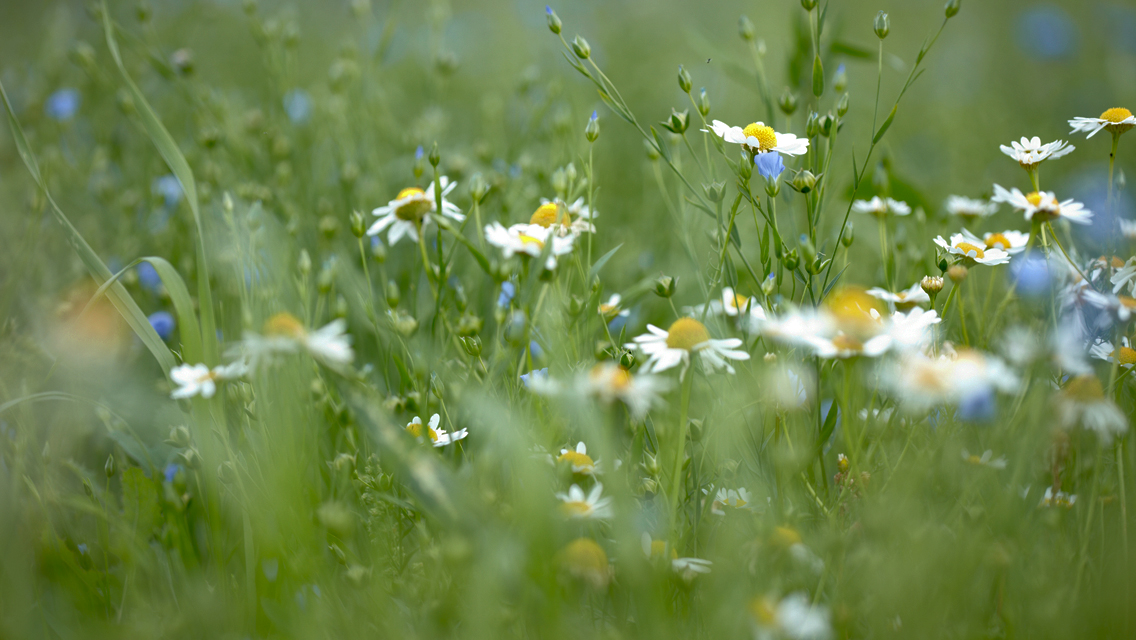
\includegraphics[width=12cm]{Daisy.jpg}| 的命令可以纳入图片.

如图 \ref{fig:1} 是一个纳入~jpg 图片的例子.

\begin{figure}[h]
\centering
  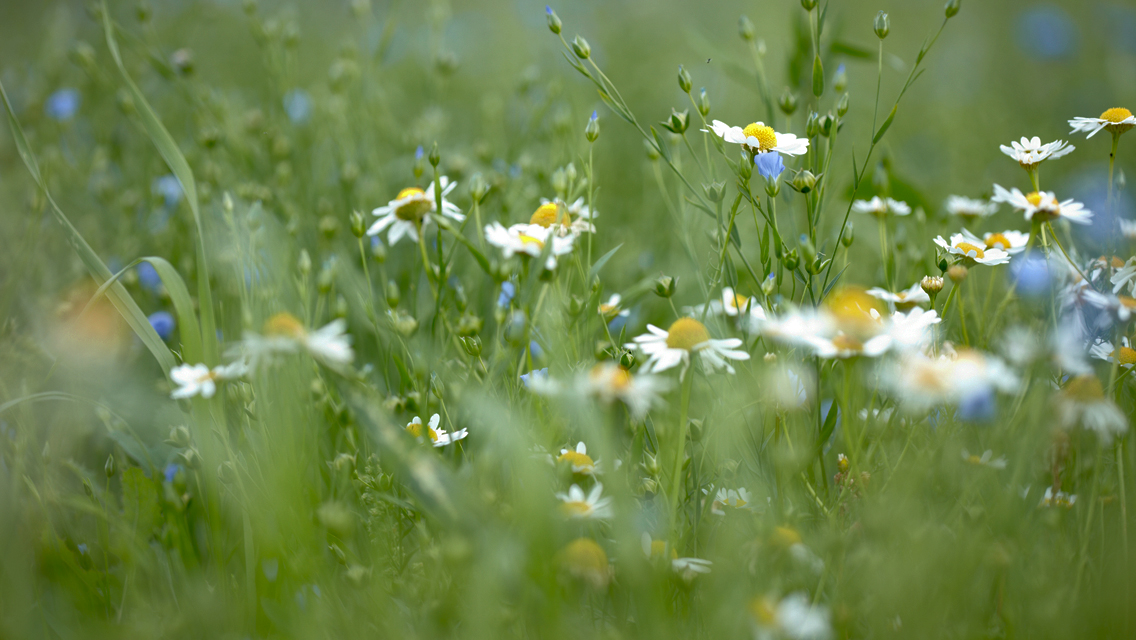
\includegraphics[width=12cm]{Daisy.jpg}
  \caption{一个彩色 jpg 图片的例子}
  %英文标题begin
  \addtocounter{figure}{-1}
  \vspace{-5pt}
  %\SetEnglishCaption
  \renewcommand{\figurename}{Figure}
  \caption{An example of a color jpg image}
  \renewcommand{\figurename}{图}
  \label{fig:1}
\end{figure}

表格问题, 建议使用``三线表'', 如表 \ref{tab:1}.

\begin{table}[h]
\centering
\caption{一般三线表}
%英文标题begin
\addtocounter{table}{-1}
\vspace{-5pt}
%\SetEnglishCaption
\renewcommand{\tablename}{Table}
\caption{Three row table}
\renewcommand{\tablename}{表}
%英文标题end
\label{tab:1}
    \begin{tabular}{c c c c c c c c c c c}
    \hline
    123 & 4  & 5  & 123 & 4 & 5123 & 4 & 5 & 123 & 4 & 5\\
    \hline
    67 & 890 & 13 & 123 & 4 & 5123 & 4 & 5 & 123 & 4 & 5\\
    67 & 890 & 13 & 123 & 4 & 5123 & 4 & 5 & 123 & 4 & 5\\
    67 & 890 & 13 & 123 & 4 & 5123 & 4 & 5 & 123 & 4 & 5\\
    \hline
    \end{tabular}
\end{table}

%\begin{table}[h]
%  \centering
%  \caption{调整线宽的三线表}\label{tab:2}
%    \begin{tabular}{c c c c c c c c c c c}
%    \hlinewd{0pt}
%    姓名: &&&&年龄: &&&& 性别:\\
%    \hlinewd{1.5pt}
%    123 & 4  & 5  & 123 & 4 & 5123 & 4 & 5 & 123 & 4 & 5\\
%    \hlinewd{1pt}
%    67 & 890 & 13 & 123 & 4 & 5123 & 4 & 5 & 123 & 4 & 5\\
%    67 & 890 & 13 & 123 & 4 & 5123 & 4 & 5 & 123 & 4 & 5\\
%    67 & 890 & 13 & 123 & 4 & 5123 & 4 & 5 & 123 & 4 & 5\\
%    \hlinewd{1.5pt}
%    \end{tabular}
%\end{table}

%\section{论文电子版提交的格式问题}
%
%《武汉大学博、硕士研究生学位论文缴送办法》要求``电子版应采用~Word97 或~Word2000 格式(DOC)编辑''\footnote{那已经是~2005 年的事情了.}.
%关于这个重要的问题, 我已致信武汉大学图书馆总馆信息服务中心袁晓川老师,
%得到的答复是: ``用~\LaTeX{} 软件排版的论文可直接提交~PDF 格式.''







\chapter{其他事项}
以下是广告时间, 插播一段广告:
\begin{itemize}
    \item 插图的制作, 建议 pgf.
          pgf 的长处是源文件直接植入~\TeX~文档, 管理起来非常方便.
    这里有我写的一个关于初次使用~pgf~的帖子:\\    \url{http://bbs.ctex.org/forum.php?mod=viewthread&tid=30480}.
    \item 生成参考文献, 建议使用~BibTeX.  这里有我写的一个文档: \\
    \url{http://bbs.ctex.org/forum.php?mod=viewthread&tid=26056}.

      {\kaishu 使用 BibTeX{} 做参考文献时,
      借助 EndNote 或者 NoteExpress, 可以非常漂亮简单地解决 bib 文件的录入问题.
      NoteExpress 在校图书馆网站有正版软件提供下载.
      当然 EndNote 本身就是 Thomson Corporation 推出的(和 SCI 搜索引擎是同一家公司),
      和多个重要文献搜索引擎有良好的功能配合.

      Google 学术搜索也提供了文献的 bib 格式.
      录入参考文献时, 偶尔用一用 Google 学术搜索, 还可以核查或减少录入的错误, 并减少录入的工作量.}
     \item 幻灯片的制作, 建议使用~Beamer. 这里有我写的一个模板, 谨供参考:\\
    \url{http://bbs.ctex.org/forum.php?mod=viewthread&tid=27695}.
\end{itemize}






%%%=== 参考文献 ========%%%
\cleardoublepage\phantomsection
\addcontentsline{toc}{chapter}{参考文献}
\begin{thebibliography}{000}\zihao{5}
	\thispagestyle{onlytitle}
	
  \bibitem{r2} 作者, 书名, 年份, 版次, 出版地: 出版单位, 起止页码

  \bibitem{r1} 作者, 文章题目, 期刊名, 年份(期数): 起止页码



  \bibitem{r3} 邓建松等, 《\LaTeXe~科技排版指南》, 科学出版社

  \bibitem{r4} 吴凌云, 《CTeX~FAQ (常见问题集)》, \textit{Version~0.4}, June 21, 2004

  \bibitem{r5} Herbert Vo\ss, Mathmode, \url{http://www.tex.ac.uk/ctan/info/math/voss/mathmode/Mathmode.pdf}.

\end{thebibliography}








\backmatter
% !Mode:: "TeX:UTF-8"

%%% 此部分内容:  (1) 攻读硕士学位期间参加的科研项目  (2) 攻读硕士学位期间完成的学术成果  (3) 攻读硕士学位期间获得的奖项  (4) 致谢

%%%=== 攻读硕士学位期间参加的科研项目 ========%%%
\project
\thispagestyle{onlytitle}
\begin{enumerate}[{[1]}]
	\item   国家自然科学基金项目“链路相关无线网络中基于网络编码的数据分发机制研究”(项目编号:61502230);
\end{enumerate}


%%%=== 攻读硕士学位期间完成的学术成果 ========%%%
\achievement
\thispagestyle{onlytitle}
 \textbf{【本人或者导师作为第一作者文章】}
\begin{enumerate}[{[1]}]
	\item   \textbf{Yiren Gu(顾伊人)}, Hang Shen, Guangwei Bai, Tianjing Wang, Xuejun Liu. QoI-Aware Incentive for Multimedia Crowdsensing Enabled Learning System[J], Multimedia Systems (Springer), 2020, 26(1): 3-16, DOI 10.1007/s00530-019-006 16-w (SCI,中科院三区,CCF推荐C类期刊,篇幅14页)
	\item 国家发明专利:一种用于机器学习系统的多媒体群智感知激励方法,发明人:白光伟,\textbf{顾伊人},沈航,沙鑫磊,张杰,申请号:201910096432.X,申请日期:2019年1月31日,已受理 (第二发明人,导师为第一发明人)
\end{enumerate}
\par
 \textbf{【合作发表成果】}
\begin{enumerate}[{[1]}]
	\item   国家发明专利:一种数据质量感知的移动群智感知激励方法, 发明人:白光伟, 童海, 沈航, \textbf{顾伊人}, 胡煜家,申请号: 201910455446.6,申请日期: 2019年 05 月 29 日,已受理
\end{enumerate}


%%%=== 攻读硕士学位期间获得的奖项 ========%%%
\awards
\thispagestyle{onlytitle}
\textbf{【本人或者导师作为第一作者文章】}
\begin{enumerate}[{[1]}]
	\item 2019年12月获2019年度“硕士研究生国家奖学金”;
	\item 2019年12月评为2019年度计算机科学与技术学院“优秀共产党员”;
	\item 2019年9月评为计算机科学与技术学业“优秀部长”;
	\item 2019年9月获校研究生学业奖学金特等奖;
\end{enumerate}

%%%%%%%%%%%%%%%%%%%%%%%
%%% --------------- 致谢 ------------- - %%%
%%%%%%%%%%%%%%%%%%%%%%%
\acknowledgement
\thispagestyle{onlytitle}

感谢你, 感谢他和她, 感谢大家.

%%%%%%%%%%%%%%%%%%%%%%%%%%%%%%%%%%%%%%%
%%%%%%%--判断是否需要空白页-----------------------------
  \iflib
  \else
  \newpage
  \cleardoublepage
  \fi
%%%%%%%-------------------------------------------------







 %%%攻读硕士学位期间参加的科研项目,学术成果,奖项,致谢.
\cleardoublepage
\end{document}



